\documentclass[
a4paper, % Paper size, use either a4paper or letterpaper
12pt, % Default font size, the template is designed to look good at 12pt so it's best not to change this
%unnumberedsections, % Uncomment for no section numbering
]{article}
\usepackage[a4paper,top=0.8cm, bottom=0.8cm, left=1.6cm, right=1.6cm]{geometry}

\usepackage{cmap} % make PDF files searchable and copy-able
\usepackage[utf8]{inputenc}
\usepackage[english,russian]{babel}

\usepackage{amssymb,amsmath}
\renewcommand {\phi}{\varphi}
\usepackage{mathtext}

\usepackage{libertine}
\usepackage[libertine]{newtxmath}

\usepackage{graphicx} % Required for inserting images
\graphicspath{{./img/}} % Destination of images
\usepackage{subcaption}

\usepackage{hyperref}

\usepackage{xcolor}

% opening
\title{
	\textcolor{cyan}{Отчет о выполнении лабораторной работы 2.2.1}
	\\
	Исследование взаимной диффузии газов
}
\author{Шубин Владислав, Байбулатов Амир}
%\date{Сентябрь 2023}

\begin{document}    
	
	\maketitle
	
	\section{Аннотация}
	В работе исследуется явление взаимной диффузии газов, путём регистрации зависимости концентрации гелия в воздухе от времени с помощью датчиков теплопроводности при разных начальных давлениях смеси газов. Также определяется коэффициент диффузии по результатам измерений.
	
	\newpage
	
	\section{Теоретические сведения}
	
	Диффузией называют самопроизвольное взаимное проникновение веществ друг в друга, происходящее вследствие хаотичного теплового движения молекул. При перемешивании молекул разного сорта говорят о взаимной (или концентрационной) диффузии.
	
	Диффузия в системе, состоящей из двух компонентов $ a $ и $ b $ (бинарная смесь), подчиняется закону Фика: плотности потока компонентов $ j_{a,b} $ (количество частиц, пересекающих единичную площадку в единицу времени) пропорциональны градиентам их концентраций $ \nabla n_{a,b}$, что в одномерном случае можно записать как
	
	\[ j_a = -D\dfrac{\partial n_a}{\partial x}, \quad j_b = -D\dfrac{\partial n_b}{\partial x}, \]
	где $ D $ -- коэффициент взаимной диффузии компонентов. Знак <<минус>> отражает тот факт, что диффузия идёт в направлении выравнивания концентраций. Равновесие достигается при равномерном распределении вещества по объёму сосуда ($ \partial n / \partial x = 0 $).
	
	В случае работы с данной установкой можно считать, что диффузионный поток одинаков в любом сечении трубки, соединяющей сосуды $V_1$ и $V_2$. Следовательно:
	
	\begin{align}
		J = -DS\dfrac{n_1-n_2}{l} \qquad DS\frac{n_1-n_2}{l} = -V_1\dfrac{dn_1}{dt} = V_2\dfrac{dn_2}{dt} \\
		\dfrac{dn_1 - dn_2}{dt} = -\dfrac{n_1-n_2}{l}DS\left(\dfrac{1}{V_1}+\dfrac{1}{V_2}\right) \quad\Rightarrow\quad n_1-n_2 = (n_1-n_2)_0e^{-\dfrac{t}{\tau}}
	\end{align}
	
	В данной работе исследуется взаимная диффузия гелия и воздуха. Давление P и температура T в условиях опыта предполагаются неизменными: $ p=(n_{He}+n_{\text{в}})kT $, где $ n_{He} $ и $ n_{\text{в}} $ -- концентрации (объёмные плотности) диффундирующих газов. Поэтому для любых изменений концентраций справедливо $ \Delta n_{He}=-\Delta n_{\text{в}} $. Следовательно, достаточно ограничиться описанием диффузии одного из компонентов, например гелия $ n_{He} $:
	
	\begin{equation}\label{1}
		j_{He}=-D\dfrac{\partial 	n_{He}}{\partial x}.
	\end{equation}
	
	Приведём теоретическую оценку для коэффициента диффузии. В работе концентрация гелия, как правило, мала $ (n_{He} \ll n_\text{в}) $. Кроме того, атомы гелия существенно легче молекул, составляющих воздух ($ \mu_{He} \ll \mu_{O_2}, \mu_{N_2} $), значит и их средняя тепловая скорость велика по сравнению с остальными частицами. Поэтому перемешивание газов в работе можно приближенно описывать как диффузию примеси лёгких частиц $ He $ на практически стационарном фоне воздуха. Коэффициент диффузии в таком приближении равен
	
	\begin{equation}\label{2}
		D=\dfrac{1}{3}\lambda 	\overline{v},
	\end{equation}
	
	где $ \overline{v}=\sqrt{\frac{8RT}{\pi \mu}} $ -- средняя тепловая скорость частиц примеси, $ \lambda = \frac{1}{n_0\sigma} $ -- их длина свободного пробега, $ n_0 $ -- концентрация рассеивающих центров (фона), $ \sigma $ -- сечение столкновения частиц примеси с частицами фона.
	
	Таким образом, теория предсказывает, что коэффициент диффузии бинарной смеси обратно пропорционален давлению в системе $ D \propto 1/P $, и не зависит от пропорций компонентов, что и предлагается проверить в работе экспериментально.
	
	\newpage
	
	\section{Оборудование и инструментальные погрешности}
	\textbf{Оборудование:} манометр, вольтметр, форвакуумный насос, 2 сосуда.
	% \begin{itemize}
		% 	\item \textbf{Манометр}: $\Delta = $ (по цене деления)
		% 	\item \textbf{Вольтметр}: $\Delta m = \pm{5}$ мг (маркировка производителя)
		% \end{itemize}
	
	\section{Результаты измерений и обработка данных}
	
	\subsection{Экспериментальная установка}
	
	Для исследования взаимной диффузии используется следующая установка:
	
	\begin{figure}[h!]
		\centering
		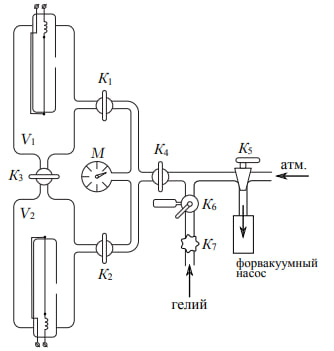
\includegraphics[width=0.5\linewidth]{img/experiment_scheme.jpg}
		\caption{Схема установки}
		\label{fig:enter-label}
	\end{figure}
	Здесь $V_1,\; V_2$ -- два сосуда с примерно равным объемом, в которые мы будем загонять воздух и гелий.
	
	Данная конструкция позволяет провести диффузию, которая возможна только при равенстве давлений.
	
	Основное оборудование, с помощью которого мы будем снимать измерения -- датчики теплопроводности, через которые пропускают ток. Они подключены к мосту, который позволяет нам устанавливать начальное равновесное состояние.
	
	При изменении концентрации в колбах вольтметр покажет нам разность напряжений на датчиках, что, из-за их конструкции, означает разность концентраций. 
	
	С помощью изменения напряжения мы и будем изучать процесс диффузии, т.к. во время ее протекания концентрации газов начинают устанавливаться, что заметно на графике разницы напряжений от времени.
	
	\textbf{Особенности установки}
	
	Кран К4 обладает повышенной вакуумплотностью и используется для изолирования измерительной части установки от возможных протечек гелия и воздуха. Двухходовой кран К5 служит для подключения форвакуумного насоса к установке, подачи воздуха в установку и соединения форвакуумного насоса с атмосферой. Устройство и назначение кранов К6 и К7 подачи гелия соответствуют основному описанию.
	
	\subsection{Характеристики системы}
	
	$V = 800 \pm 5 \:\: \text{см}^3$ \\
	$\dfrac{L}{S} = 15,0\pm 0,1 \:\: \text{см}^{-1}$. 
	
	\newpage
	
	\subsection{Измерения:}
	
	%\newpage
	\subsubsection{Коэффицент взаимной диффузии}
	
	Для смеси гелий-воздух исследуем зависимость коэффициента взаимной диффузии о начального давления в системе. Для этого будем фиксировать с помощью компьютера в лаборатории зависимость показаний вольтметра от времени, прошедшего с начала эксперимента. Проверим то, что процесс диффузии подчиняется закону: \[U = (U)_0e^{-\dfrac{t}{\tau}}.\]
	
	Для этого построим графики зависимости в виде:
	\begin{align}
		\ln(U) = \ln(U_0) + (-\tau^{-1})t \Rightarrow \ln\left(\frac{U_0}{U}\right) = \frac{t}{\tau}
	\end{align}
	
	\begin{figure}[h!]
		\centering
		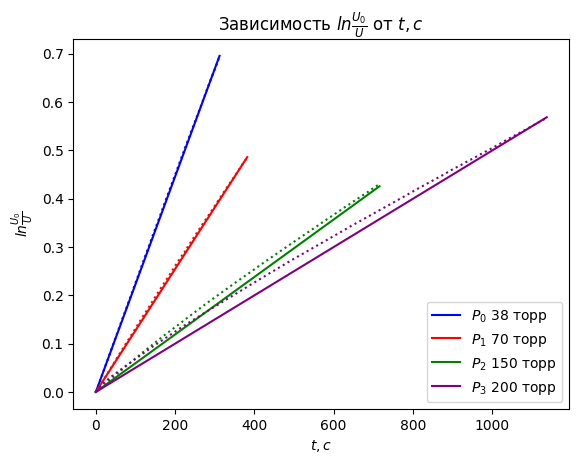
\includegraphics[width=0.8\linewidth]{img/graph.png}
		\caption{Зависимость $ \ln\frac{U_0}{U} $ от $ t $}
		\label{fig:graph}
	\end{figure}
	
	График \ref{fig:graph} линеен, следовательно у нас происходит действительно диффузия. Далее мы можем найти $\tau$ как коэффицент наклона. Находить будем по МНК. В нашем случае $\ln\frac{U_0}{U} = k t$, и $k = \frac{1}{\tau}$.
	
	\begin{equation}
		k=\frac{\langle t\cdot \ln \frac{U_0}{U} \rangle - \langle t\rangle \langle \ln \frac{U_0}{U}\rangle}{\langle t^2 \rangle - \langle t \rangle^2} 
	\end{equation}
	\begin{equation}
		\sigma_k^\text{случ}=\frac{1}{\sqrt{N}}\sqrt{\frac{\langle \left(\ln\frac{U_0}{U}\right)^2 \rangle - \langle \ln\frac{U_0}{U} \rangle^2}{\langle t^2 \rangle - \langle t \rangle^2} - k^2  }
	\end{equation}
	\begin{equation}
		\sigma_k^{\text{сист}} = k\varepsilon_k =  k\cdot\sqrt{\varepsilon_{U_0}^2 + \varepsilon_U^2 + \varepsilon_t^2} = k\cdot\sqrt{\left(\frac{\sigma_{U_0}}{U_0}\right)^2+ \left(\frac{\sigma_{U}}{U}\right)^2 + \left(\frac{\sigma_t}{t}\right)^2} 
	\end{equation}
	\begin{equation}
		\sigma_k = \sqrt{\left( \sigma_k^\text{случ} \right)^2 + \left( \sigma_k^\text{сист} \right)^2 }
	\end{equation}
	
	\newpage
	
	Проведем рассчеты для каждого значения давления, получим таблицу:
	
	\begin{table}[h!]
		\centering
		\begin{tabular}{|c|c|c|c|c|}
			\hline
			$ P $, торр & $ k \cdot 10^{-3} $, с$ ^{-1} $ & $ \sigma_{k} \cdot 10^{-3} $, с$ ^{-1} $ & $ \tau $, с & $ \sigma_\tau $, с \\ \hline
			38 & 2,22 & 0,09 & 449,1 & 3,1 \\ \hline
			70 & 1,27 & 0,08 & 786,5 & 6,1  \\ \hline
			150 & 0,59 & 0,03 & 1682,9 & 7,2  \\ \hline
			200 & 0,48 & 0,01 & 2073,0 & 11,0 \\ \hline
		\end{tabular}
		\caption{Аппроксимация зависимостей}
		\label{tab:approx}
	\end{table}
	
	Далее посчитаем коэффициенты взаимной диффузии для различных давлений по формуле:
	\begin{align}
		D = \frac{1}{\tau}\frac{VL}{2S} & & \sigma_D = D\sqrt{\varepsilon_\tau^2 + \varepsilon_V^2  + \varepsilon_{\frac{L}{S}}^2}
	\end{align}
	
	Посчитаем $D\text{ и }\sigma_D$:
	
	\begin{table}[h!]
		\centering
		\begin{tabular}{|c||c|c|c|c|}
			\hline
			$ P $, торр & 38 & 70 & 150 & 200 \\
			\hline
			$ D $, $\dfrac{\text{см}^2}{\text{с}}$ & 4,57 & 2,61 & 1,22 & 0,99 \\
			\hline
			$ \sigma_D $, $\dfrac{\text{см}^2}{\text{с}}$ & 0,13 & 0,08 & 0,07 & 0,06\\
			\hline
		\end{tabular}
		\caption{Значения коэффициента диффузии при различных давлениях}
		\label{tab:D}
	\end{table}
	
	\subsection{График зависимости $D(\dfrac{1}{P})$}
	
	\begin{figure}[h!]
		\centering
		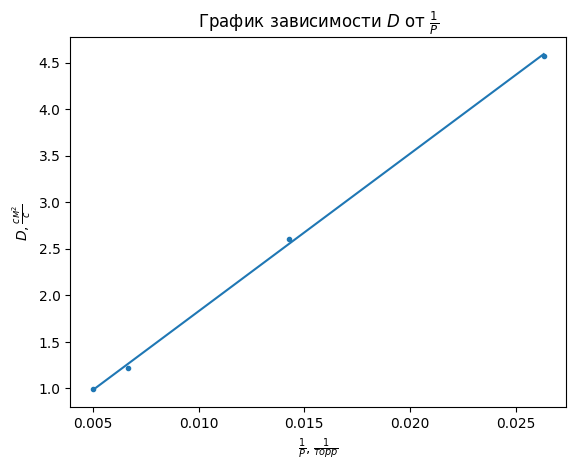
\includegraphics[width=0.5\linewidth]{img/2ndgraph.png}
		\caption{Зависимость $ D $ от $ \dfrac{1}{P}$}
		\label{fig:2nd_graph}
	\end{figure}
	
	Построен по МНК, коэффицент наклона $k = (410,2\pm19,1)\text{ } \frac{\text{см}^2}{\text{с}\cdot\text{торр}}$. 
	
	Значит, коэффициент диффузии при атмосферном давлении можно найти таким образом:\[D_\text{атм} = k\dfrac{1}{P_\text{атм}} = (0,545\pm0,03)\text{ } \frac{\text{см}^2}{\text{с}}\]
	
	\subsubsection{Длина свободного пробега}
	По полученным данным оценим длину свободного пробега атомов гелия в воздухе:
	
	\begin{align}
		D=\dfrac{1}{3}\lambda\langle v\rangle,\text{ где } \langle v \rangle = \sqrt{\dfrac{8RT}{\pi \mu}} \Rightarrow \lambda = 3D\sqrt{\dfrac{\pi \mu}{8RT}} \approx 140,3\text{ нм}
	\end{align}
	
	
	\section{Заключение}
	В ходе работы:
	
	\begin{itemize}
		\item Была зарегистрирована зависимость концентрации гелия в воздухе от времени с помощью датчиков теплопроводности при различных начальных давлениях смеси газов.
		\item По результатам измерений был определен коэффицент взаимной диффузии для смеси гелий-воздух: $D_\text{атм} = (0,545\pm0,03)\text{ } \frac{\text{см}^2}{\text{с}}$, что совпадает по порядку величины с табличными данными: $D_\text{табл} = 0,62\text{ } \frac{\text{см}^2}{\text{с}}$.
		\item Была оценена длина свободного пробега гелия в воздухе: $\lambda = (140,3\pm7,5)\text{ нм}$, что опять-таки сходится с табличными данными по  порядку величины: $\lambda_\text{табл} = 175\text{ нм}$. 
	\end{itemize}
	Основная доля ошибок приходится на барометр, и тот факт, что мы не можем полностью точно сбалансировать мост (он очень легко расстраивается).
	
\end{document}